\documentclass[12pt,a4paper,twocolumn]{article}
\usepackage[margin=2cm,columnsep=0.8cm]{geometry}
\usepackage{setspace}
\usepackage{authblk}
\usepackage{graphicx}
\usepackage{subcaption}
\usepackage{float}
\usepackage{booktabs}
\usepackage{amsmath,amsfonts,amssymb}
\usepackage{siunitx}
\usepackage[round,sort&compress]{natbib}
\usepackage{hyperref}
\usepackage{caption}
\usepackage{fancyhdr}
\usepackage{xcolor}
\usepackage{libertine}
\captionsetup{font=small,labelfont=bf}
\pagestyle{fancy}

\graphicspath{{results/}{../results/}{./}}

\fancyhf{}
\fancyhead[L]{\textit{Opinion vs.\ Fact Classification}}
\fancyhead[R]{\thepage}

\title{Opinion vs.\ Fact Classification:\\ A Two-Stage NLP Pipeline}
\author[1]{Can Duyar}
\author[1]{Daniel Ainikkal}
\affil[1]{Graz University of Technology, Graz, Austria --- Group 55}
\date{\today}

\begin{document}
\maketitle

\begin{abstract}
We address the task of deciding whether a short text states a fact or expresses
an opinion, building two deliberately separate pipelines as required by the
project brief. Stage~1 stays within traditional NLP: we hand-craft 49 linguistic
features (part-of-speech ratios, named-entity statistics, sentiment, readability
and stance markers) and feed them to classic machine-learning classifiers, with
no transformers involved. Stage~2 takes the LLM route, fine-tuning
\texttt{facebook/bart-base} on inputs augmented with a compact linguistic
knowledge-base tag. Each stage is measured against a baseline: a majority-class
predictor for Stage~1 and a zero-shot \texttt{bart-large-mnli} classifier for
Stage~2. On an internal stratified split of 855 labelled texts, the Stage~1
Random Forest reaches \num{0.859} F1-macro against a \num{0.341} majority
baseline, while the fine-tuned Stage~2 model reaches \num{0.965} F1-macro,
improving on the \num{0.472} zero-shot baseline by \num{0.493}. We find that
fine-tuning clearly outperforms feature engineering, but at a considerable cost
in compute and interpretability. All results are reproducible from a fixed seed.
\end{abstract}

\section{Introduction}
\label{sec:intro}
The task is to decide whether a short piece of text states a fact or expresses an
opinion. We build two separate pipelines for this, as the brief asks. Stage~1
sticks to traditional NLP: we hand-craft linguistic features and feed them to
ordinary machine-learning classifiers, with no transformers involved. Stage~2
goes the LLM route and fine-tunes BART~\citep{lewis2020bart}, with a small
linguistic knowledge base mixed into the input. Both stages are checked against a
baseline and both produce predictions for the released validation set
(\texttt{group55\_classifications\_1.csv} and
\texttt{group55\_classifications\_2.csv}). We keep the code for the two stages in
separate folders (\texttt{stage1/} and \texttt{stage2/}), with a shared
\texttt{utils.py} for loading data, normalising labels and computing metrics.
The main insights can be taken from this introduction, the results
(Section~\ref{sec:results}) and the conclusion (Section~\ref{sec:conclusion}).

\section{Related Work}
\label{sec:related}
Rather than survey the broad opinion-mining literature, we restrict our citations
to the resources our pipeline directly builds on. Stage~2 fine-tunes
BART~\citep{lewis2020bart}, a denoising sequence-to-sequence model, and reuses for
the zero-shot baseline a BART checkpoint trained on the MNLI inference
corpus~\citep{williams2018mnli}. Stage~1 draws its sentiment features from the
rule-based VADER lexicon~\citep{hutto2014vader} and is implemented with
scikit-learn~\citep{pedregosa2011scikit} and NLTK~\citep{bird2009nltk}.

\section{Materials and Methods}
\label{sec:methods}

\subsection{Dataset and preprocessing}
The labelled data (\texttt{data/dataset.csv}) has 855 rows with a
\texttt{Content} column and a \texttt{Classification} column. The labels came in
with some inconsistent casing (\texttt{OPinion}, \texttt{fact}, and so on), so we
normalise everything to \texttt{Fact} or \texttt{Opinion}. After that the split
is roughly even: 443 Fact (\SI{51.8}{\percent}) and 412 Opinion
(\SI{48.2}{\percent}), shown in Figure~\ref{fig:dist}. The separate validation
set (\texttt{validationset.csv}, 222 texts) has no gold labels, so we cannot
score on it directly. For every number we report we instead use an internal
stratified 80/20 split of the labelled data, and reserve the validation set
purely for generating the submission files. We keep preprocessing minimal: both
stages work on the raw \texttt{Content} text. A light-touch cleaner
(\texttt{utils.clean\_text}, for stripping HTML tags/entities and collapsing
whitespace) is available, but we leave the wording untouched because most of the
Stage~1 features depend on the original surface form.

\begin{figure}[t]
\centering
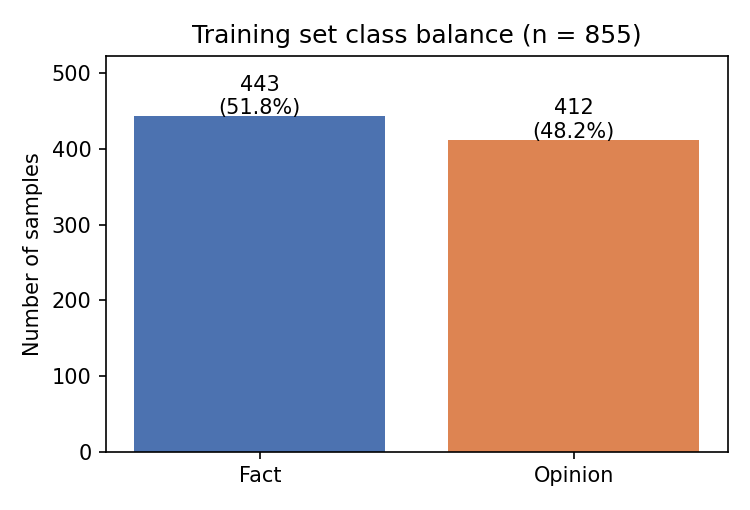
\includegraphics[width=0.85\linewidth]{report_dataset_distribution.png}
\caption{Class balance of the 855-sample training set.}
\label{fig:dist}
\end{figure}

\subsection{Stage 1: traditional NLP and classic ML}
\label{sec:m-stage1}
We turn each text into 49 numeric features
(\texttt{stage1/feature\_extractor.py}); Table~\ref{tab:feats} groups them. The
idea is simple: opinions tend to be subjective, hedged, first-person and full of
evaluative words, while facts tend to name entities, cite sources, give numbers
and use reporting verbs. Every classifier runs inside a pipeline that first
imputes missing values with the median and then standardises the features. We
compare five models with 5-fold stratified cross-validation and pick the best by
F1-macro. The baseline is a majority-class \texttt{DummyClassifier}; the learned
models are Logistic Regression, Random Forest (300 trees), Gradient Boosting
(200 trees, learning rate \num{0.05}, depth 4) and an RBF SVM, with balanced
class weights where supported.

\begin{table}[t]
\centering
\small
\begin{tabular}{@{}ll@{}}
\toprule
\textbf{Group} & \textbf{Example features (library)} \\
\midrule
POS ratios & noun/verb/adj/adv/modal/proper-noun (NLTK) \\
Named entities & PERSON/ORG/GPE counts, NER density \\
Sentiment & VADER pos/neg/neu/compound, variance \\
Readability & Flesch--Kincaid, Gunning-Fog, SMOG, ARI \\
Lexical & type--token ratio, content-word ratio \\
Opinion/Fact lexicon & curated marker counts + difference \\
Epistemic & hedging, first-person, epistemic verbs \\
Surface & exclamation/quote, numeric \& citation density \\
Complexity & subordinating conjunctions, spelling errors \\
\bottomrule
\end{tabular}
\caption{The 49 features grouped by linguistic category.}
\label{tab:feats}
\end{table}

\subsection{Stage 2: knowledge-base--augmented fine-tuning}
\label{sec:m-stage2}
Our main method fine-tunes \texttt{facebook/bart-base}
(\texttt{BartForSequenceClassification} with two labels) and prepends a short
knowledge-base tag to each input (\texttt{stage2/finetune.py},
\texttt{knowledge\_base/}). The knowledge base defines eight marker categories,
for example \texttt{opinion\_strong}, \texttt{opinion\_hedge},
\texttt{fact\_attribution}, \texttt{fact\_quantitative} and
\texttt{first\_person}. At inference time \texttt{marker\_feature\_string()}
scans the text and writes out only the categories that fire, e.g.:
\begin{quote}\small\ttfamily
[kb] opinion\_strong:1 opinion\_hedge:2 In my opinion this might be the best
film\dots
\end{quote}
So the model sees the raw sentence plus a few explicit hints about the kind of
language it contains. Zero-shot on its own is not allowed and, as the baseline
shows, not good enough here. Fine-tuning pushes BART's pretrained
representations at this particular fact/opinion boundary, and the knowledge-base
tags act as a cheap prior on a training set this small (684 examples). Training
settings: 4 epochs, batch size 8, AdamW at a learning rate of
$2\!\times\!10^{-5}$, max length 256, a \SI{10}{\percent} linear warmup and a
fixed seed of 11. For the baseline we use zero-shot
\texttt{facebook/bart-large-mnli}: it treats each text as an NLI premise and
scores the hypotheses ``This statement is a fact'' / ``\dots\ an opinion'', with
no training~\citep{williams2018mnli}.

\section{Results}
\label{sec:results}

\paragraph{Stage 1.}
The four learned models all land around F1-macro \numrange{0.85}{0.86} and leave
the \num{0.341} majority baseline far behind (Table~\ref{tab:s1},
Figure~\ref{fig:s1cmp}). We went with Random Forest as the Stage~1 model: it
scored highest, if only just, and it gives readable feature importances. Those
importances line up with what we expected: the strongest signals are the
numeric-token and number-density features (facts cite figures and statistics),
followed by content-word ratio, the share of neutral-sentiment text and noun
ratio, while the opinion-minus-fact lexicon count and hedging ratio contribute
further down. The validation predictions go to
\texttt{group55\_classifications\_1.csv}.

\begin{table}[t]
\centering
\small
\begin{tabular}{@{}lc@{}}
\toprule
\textbf{Model} & \textbf{F1-macro (5-fold CV)} \\
\midrule
\textbf{Random Forest} (selected) & \textbf{\num{0.859}} \\
Logistic Regression & \num{0.857} \\
SVM (RBF) & \num{0.853} \\
Gradient Boosting & \num{0.852} \\
Majority baseline & \num{0.341} \\
\bottomrule
\end{tabular}
\caption{Stage 1 cross-validation results.}
\label{tab:s1}
\end{table}

\paragraph{Stage 2.}
On the internal \SI{20}{\percent} hold-out, fine-tuning takes F1-macro from
\num{0.472} (zero-shot) up to \num{0.965}, a jump of \num{0.493}
(Table~\ref{tab:s2}, Figure~\ref{fig:s2}). The confusion matrices make the
difference clear: the baseline keeps calling facts opinions (Fact recall only
\num{0.27}), whereas the fine-tuned model is roughly even on both classes
(\num{0.97}/\num{0.96}). The learning curve flattens after the first epoch, so
four epochs are more than enough. Predictions are saved to
\texttt{group55\_classifications\_2.csv}.

\begin{table}[t]
\centering
\small
\begin{tabular}{@{}lcc@{}}
\toprule
\textbf{Method} & \textbf{Accuracy} & \textbf{F1-macro} \\
\midrule
Zero-shot BART-MNLI (baseline) & \num{0.497} & \num{0.472} \\
\textbf{Fine-tuned BART + KB} & \textbf{\num{0.965}} & \textbf{\num{0.965}} \\
\bottomrule
\end{tabular}
\caption{Stage 2 results on the internal \SI{20}{\percent} validation split.}
\label{tab:s2}
\end{table}

\begin{figure*}[t]
\centering
\begin{subfigure}{0.48\textwidth}
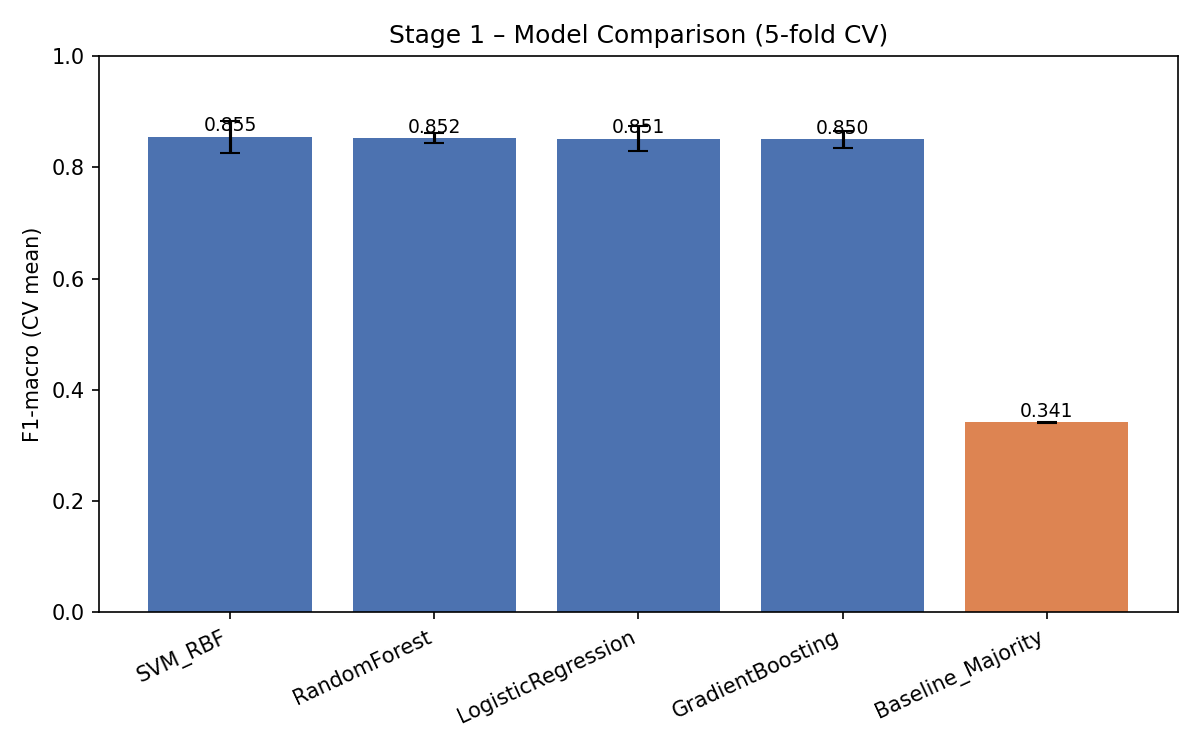
\includegraphics[width=\linewidth]{stage1_model_comparison.png}
\caption{Stage 1 CV model comparison.}
\end{subfigure}\hfill
\begin{subfigure}{0.48\textwidth}
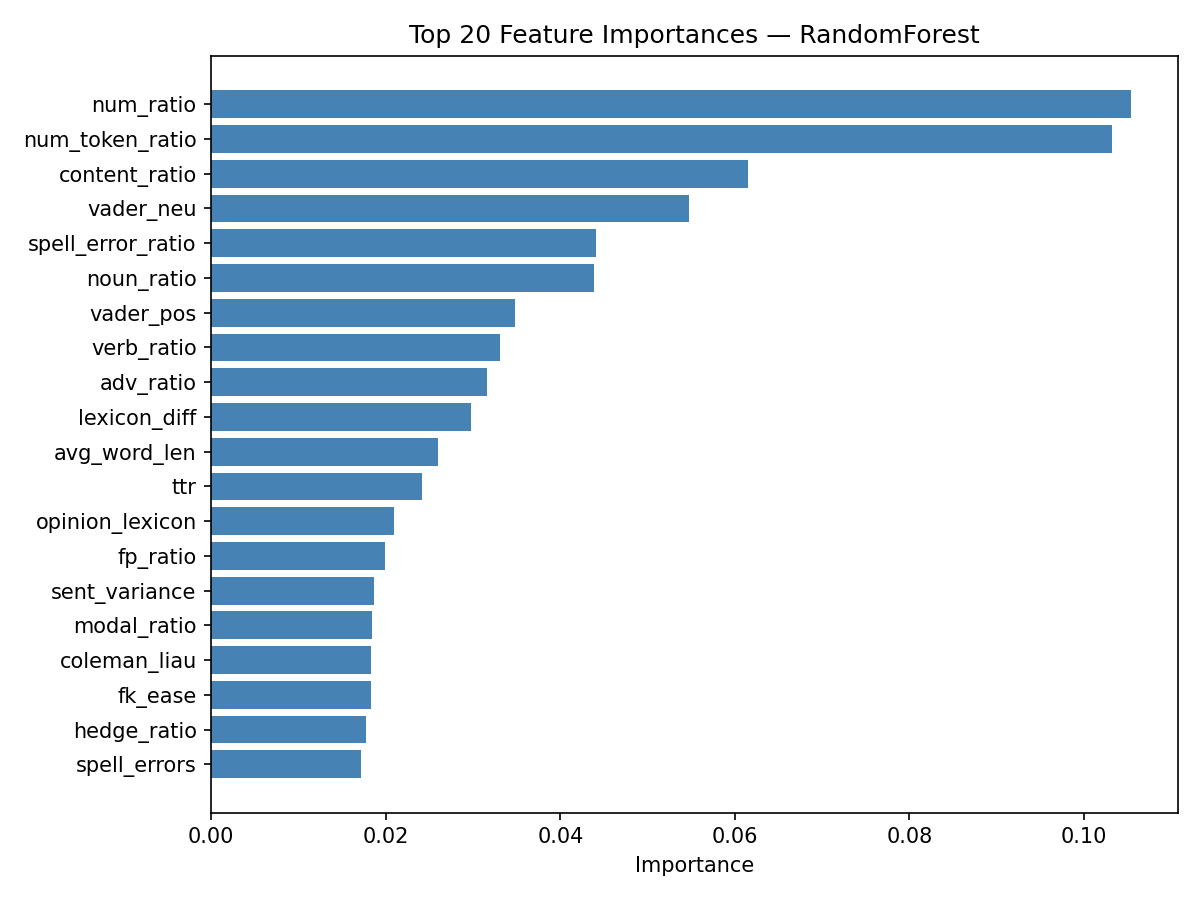
\includegraphics[width=\linewidth]{stage1_RandomForest_feature_importance.png}
\caption{Top Random-Forest feature importances.}
\end{subfigure}
\caption{Stage 1: model comparison (left) and feature importances (right).}
\label{fig:s1cmp}
\end{figure*}

\begin{figure*}[t]
\centering
\begin{subfigure}{0.40\textwidth}
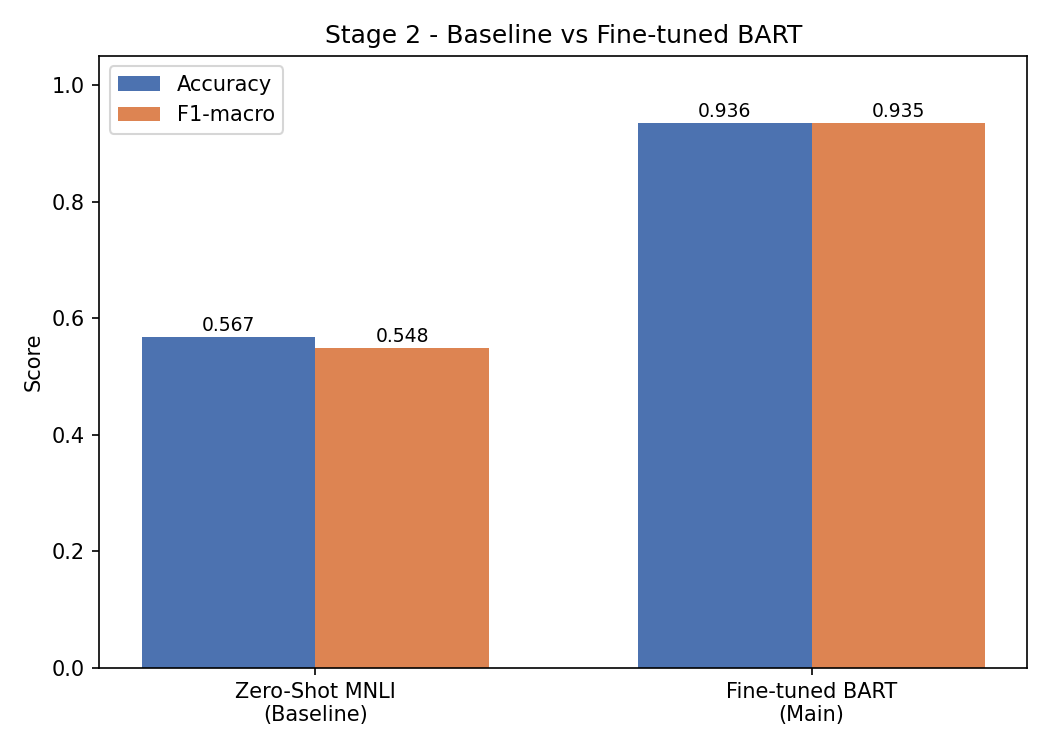
\includegraphics[width=\linewidth]{stage2_comparison.png}
\caption{Baseline vs.\ fine-tuned.}
\end{subfigure}\hfill
\begin{subfigure}{0.28\textwidth}
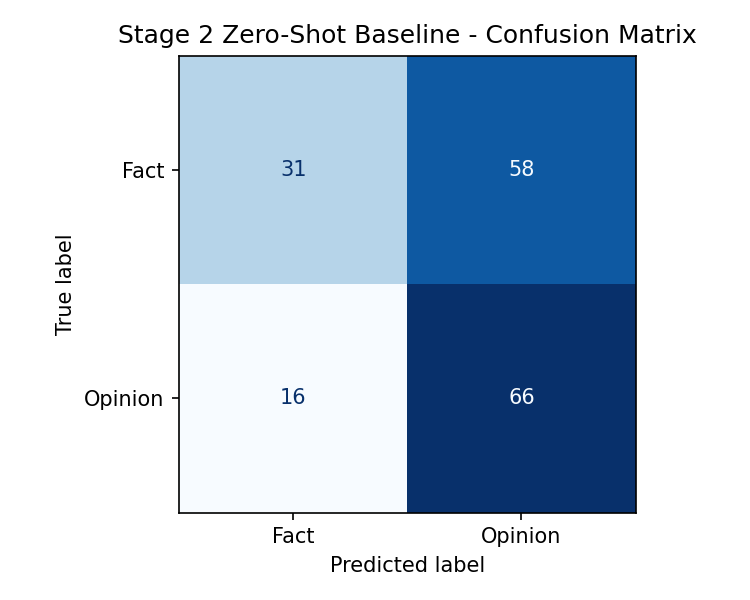
\includegraphics[width=\linewidth]{stage2_baseline_cm.png}
\caption{Zero-shot baseline.}
\end{subfigure}\hfill
\begin{subfigure}{0.28\textwidth}
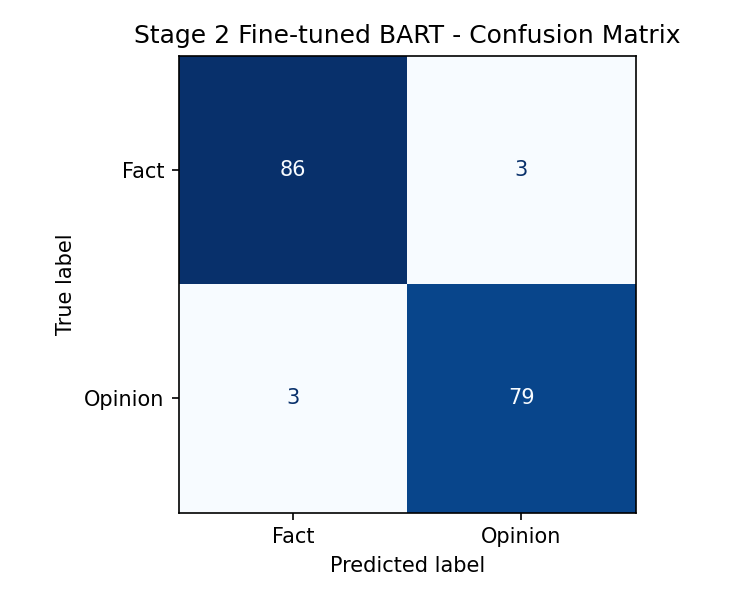
\includegraphics[width=\linewidth]{stage2_finetuned_cm.png}
\caption{Fine-tuned model.}
\end{subfigure}
\caption{Stage 2: scores (left) and confusion matrices for the zero-shot
baseline (centre) and fine-tuned model (right).}
\label{fig:s2}
\end{figure*}

\section{Discussion}
\label{sec:discussion}
Both stages beat their baselines by a wide margin (Figure~\ref{fig:summary}). The
fine-tuned LLM (\num{0.965}) comes out ahead of the feature-based Random Forest
(\num{0.859}), but it is not a free win: Stage~1 trains in seconds on a CPU and
we can explain every prediction from its features, whereas Stage~2 needs a
140M-parameter model and over an hour of CPU fine-tuning. The two scores are also
not perfectly comparable, since Stage~1 uses 5-fold CV and Stage~2 a single
\SI{20}{\percent} hold-out, and neither can be confirmed on the official set
because it has no labels. One thing worth noting is that the two stages lean on
overlapping sets of linguistic markers --- hedges, evaluative words, attribution
phrases --- even though each maintains its own lexicon rather than sharing a
single one. A further, more pragmatic difference is robustness: because Stage~2
is a fine-tuned classifier rather than a prompted generative model, it is
structurally immune to the instruction-style prompt injections that appear in the
input texts --- it can only ever output \texttt{Fact} or \texttt{Opinion}.

\begin{figure}[t]
\centering
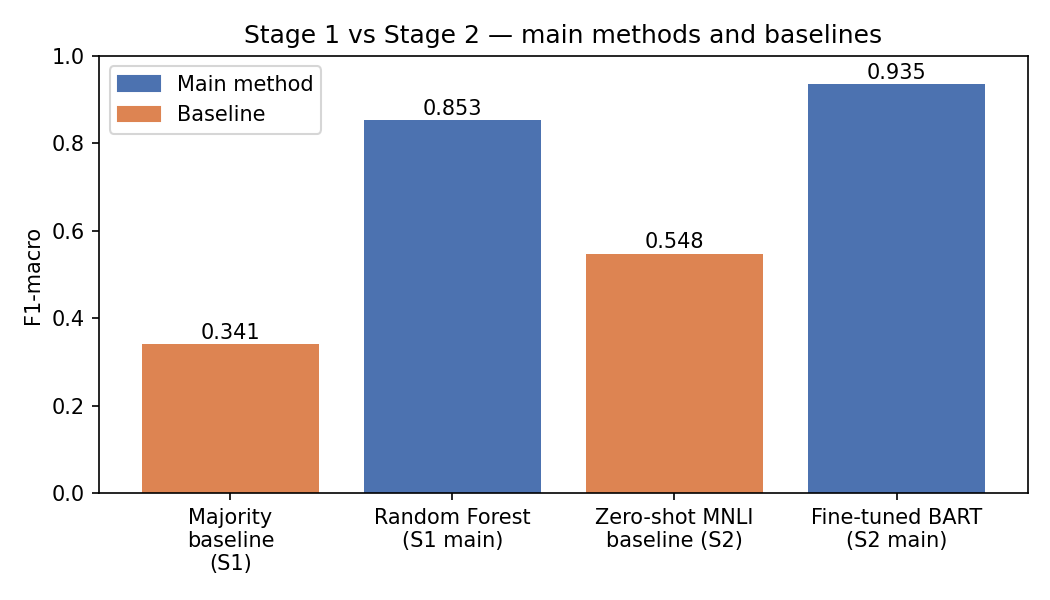
\includegraphics[width=\linewidth]{report_stage_summary.png}
\caption{F1-macro of each stage's main method and baseline.}
\label{fig:summary}
\end{figure}

\section{Conclusion}
\label{sec:conclusion}
We ended up with two clearly separated pipelines, each measured against a
baseline. Stage~1 reaches \num{0.859} F1-macro using linguistic features and a
Random Forest, and stays fully interpretable. Stage~2 reaches \num{0.965} by
fine-tuning BART on inputs that carry a small knowledge-base tag, which is a
stronger and better-justified option than relying on zero-shot prompting. If we
had more time the obvious next steps would be a proper cross-validation for
Stage~2 and a closer look at the cases both models still get wrong, such as
attributed opinions (``Experts believe X'') and promotional copy that mimics
factual phrasing.

% Everything up here counts for the page limit
\newpage

\section*{Limitations}
Our evaluation rests on a single dataset of English texts, so we cannot claim the
results transfer to other languages or domains. The official validation set has
no gold labels, so the reported numbers come from internal splits only; Stage~2
in particular uses a single \SI{20}{\percent} hold-out rather than full
cross-validation. The labelled data also contains a small number of duplicate
texts, which a random split can place in both train and evaluation, mildly
inflating Stage~2. Finally, two features are deliberately crude: the
spelling-error count is a noisy informality proxy rather than a true
spell-checker, and the knowledge-base marker matching uses substring counting,
so short markers can fire inside longer words.

\section*{Ethical Considerations}
Automated fact/opinion labelling could be misused, for instance to flag or
suppress subjective speech; our system is intended as a study aid, not a
moderation tool, and its predictions should not be treated as ground truth.
On sustainability: Stage~1 trains in seconds on a CPU, whereas Stage~2 fine-tunes
a 140M-parameter model for roughly \SI{1.5}{\hour} on a CPU per full run, a
modest but non-zero energy cost that we kept low by using the small
\texttt{bart-base} checkpoint and only four epochs. We also note that the
dataset's provenance and label correctness were taken as given; in a deployment
setting these would need independent verification.

\section*{Contributions}
\begin{table}[h!]
\centering
\caption{List of contributions per team member.}
\label{tab:contributions}
\begin{tabular}{lp{4.5cm}}
\toprule
\textbf{Team Member} & \textbf{Contribution} \\
\midrule
Can Duyar       & Base coding and report review. \\
Daniel Ainikkal & Code review and report.        \\
\bottomrule
\end{tabular}
\end{table}

\clearpage
\bibliographystyle{plainnat}
\bibliography{bibliography}

\appendix

\section{Appendix - What we tried and dropped}
For Stage~1, the other three learned models were genuine candidates, but since
they all sat within about \num{0.007} F1-macro of Random Forest, a voting
ensemble felt like effort for nothing measurable; we also tested Gaussian Naive
Bayes and a voting classifier early on, and neither helped. For Stage~2, we set
up a few-shot prompting variant that uses the knowledge base directly (16
hand-written examples with rationales plus TF-IDF retrieval, stored in
\texttt{knowledge\_base.json}). It came out weaker than fine-tuning and is much
slower at inference, so we kept only zero-shot, as the required baseline.

\section{Appendix - Usage of AI}
Generative AI assistance was used for drafting and editing prose and for code
scaffolding; all reported numbers were produced by the committed pipeline and
verified against the code. See the TU Graz guidance:
\href{https://www.tugraz.at/fileadmin/Studierende\_und\_Bedienstete/Information/Unsere\_TU\_Graz/Lehre\_an\_der\_TU\_Graz/Zitiervorschlaege_KI.pdf}{Zitiervorschlaege AI}.

\section{Appendix - Reproducibility}
All randomness is seeded (\texttt{random\_state}/\texttt{set\_seed} $=11$). The
full pipeline is reproducible with
\texttt{python run\_all.py -{}-train data/dataset.csv -{}-test
data/validationset.csv}.

\end{document}
